\documentclass[UTF8]{ctexart} %使用ctex包,中文支持
\usepackage{amsmath}  %数学公式
\usepackage{graphicx} %插图
\usepackage{fancyhdr} %个性化页眉页脚
\usepackage{geometry} %页边距
\usepackage{bm}  % 公式加粗
\usepackage{float} %为了在分栏下插入图片
\usepackage{ulem}  % 换行下划线
%\usepackage{setspace} %行间距
\usepackage{multicol} %用于实现在同一页中实现不同的分栏
\geometry{a4paper,left=2cm,right=2cm,top=2cm,bottom=2cm} % 页边距设置

\title{GAN笔记}
\author{宋佳欢}
\pagestyle{plain}

\begin{document}
	\maketitle
	\tableofcontents
	\songti \zihao{-4}
	\section{基本知识}
	
	生成器的输出的分布要与真实数据的分布越接近越好,KL散度越小越好	
	\begin{figure}[H]
	\centering
	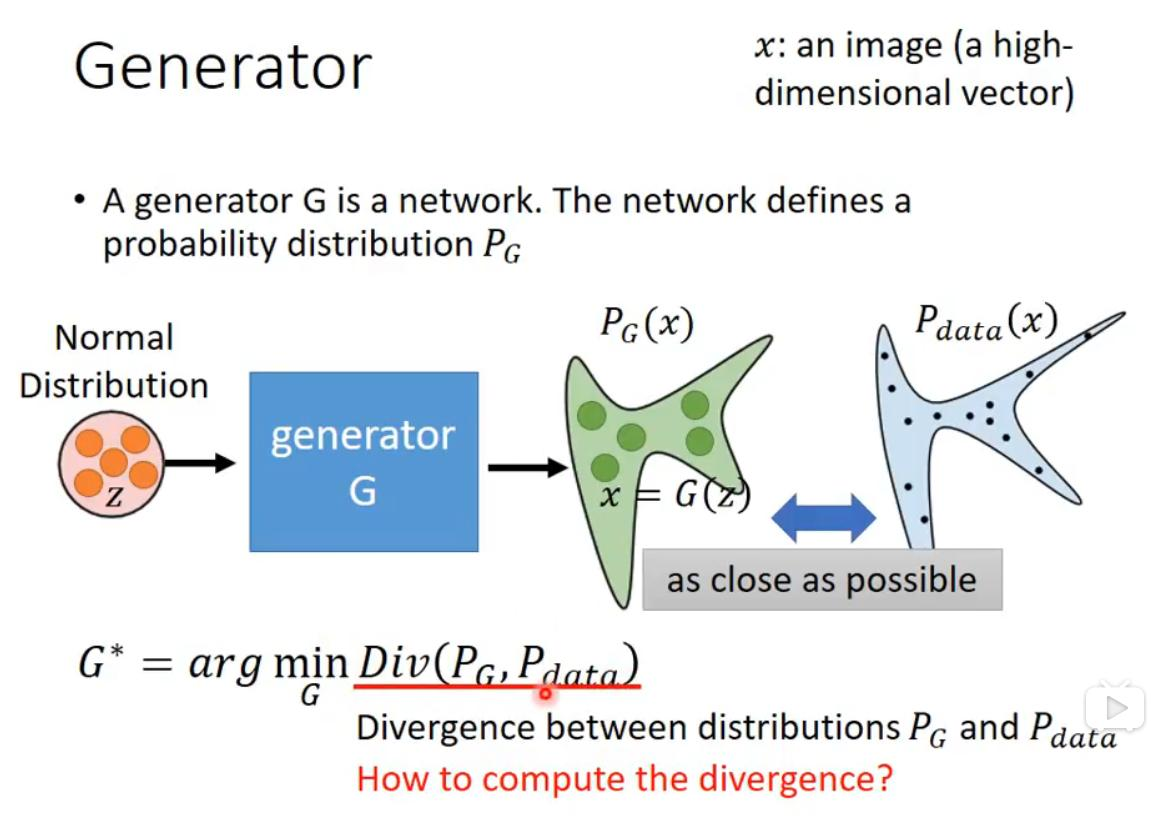
\includegraphics[scale=0.5]{screenshot001}
	\caption{生成器}
	\label{fig:screenshot001}
	\end{figure}
	但是生成器的分布表达式未知,真实数据的分布表达式也未知。所以无法代入计算KL散度,就无法优化。
	
	所以使用判别器来计算两个分布之间的差距。可以看做为一个二分类问题:
	\begin{figure}[H]
	\centering
	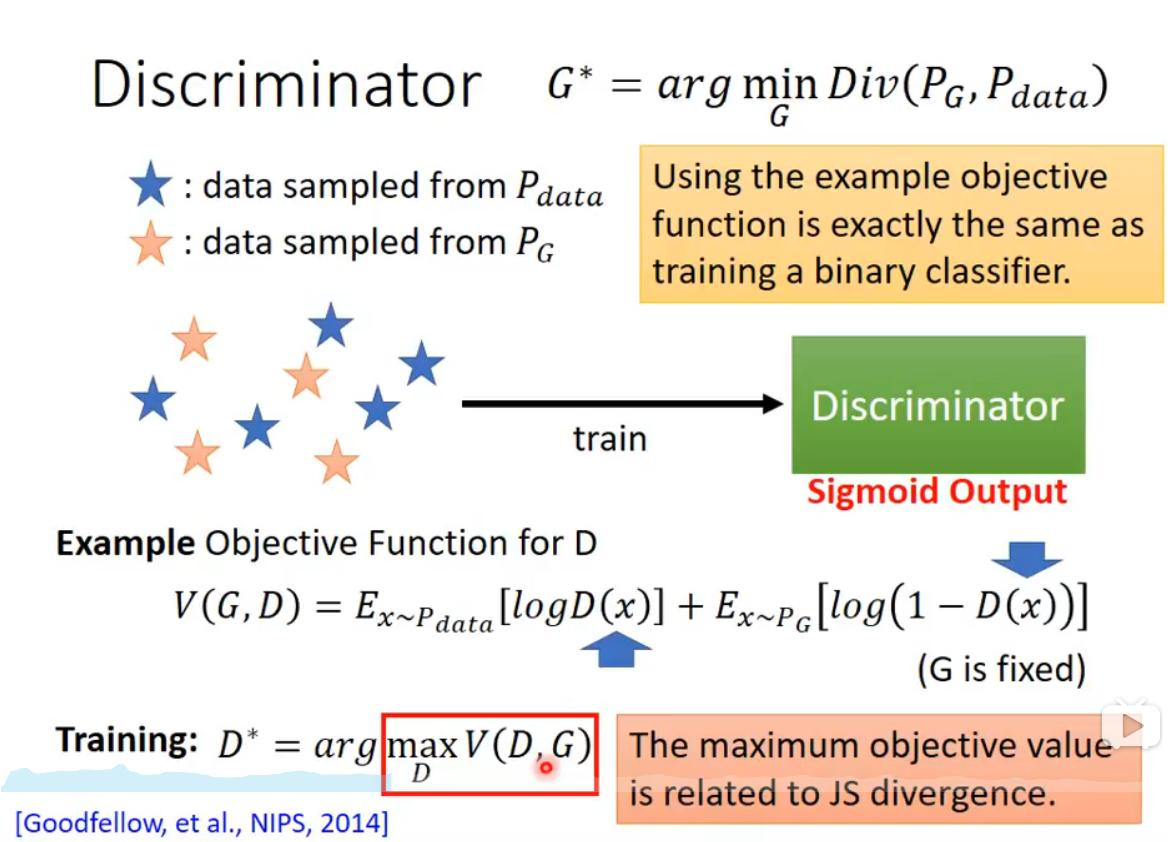
\includegraphics[scale=0.5]{screenshot002}
	\caption{判别器}
	\label{fig:screenshot002}
	\end{figure}
	判别器最大化上式目标函数$V(D,G)$,等效于最大化JS散度。
	\begin{figure}[H]
	\centering
	\caption{}
	\label{fig:screenshot003}
	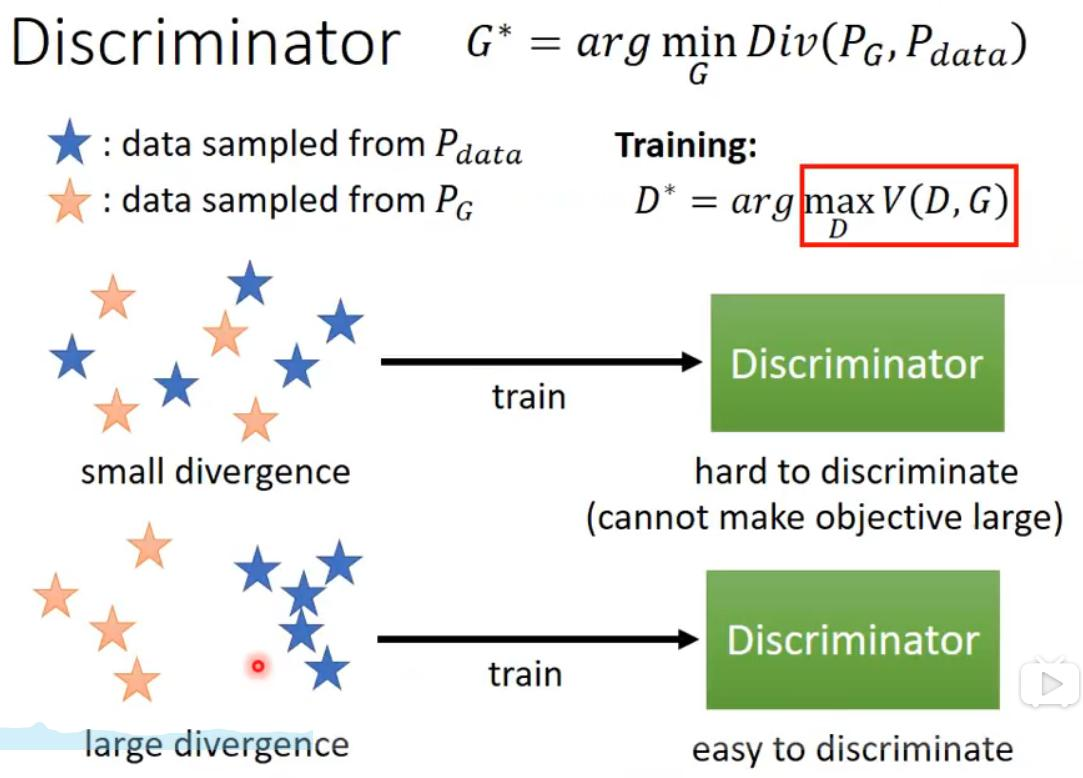
\includegraphics[scale=0.5]{screenshot003}
	\end{figure}
	
	最大化目标函数,化简后可得:优化目标函数可以将每个输入样本x分开计算
	\begin{figure}[H]
	\centering
	\includegraphics[scale=0.5]{screenshot005}
	\caption{}
	\label{fig:screenshot005}
	\end{figure}

	为了求得使得目标函数最大的判别器的参数,对每一项求偏导:得到判别器D在单个样本x下的最优值,即局部最大值。
	\begin{figure}[H]
	\centering
	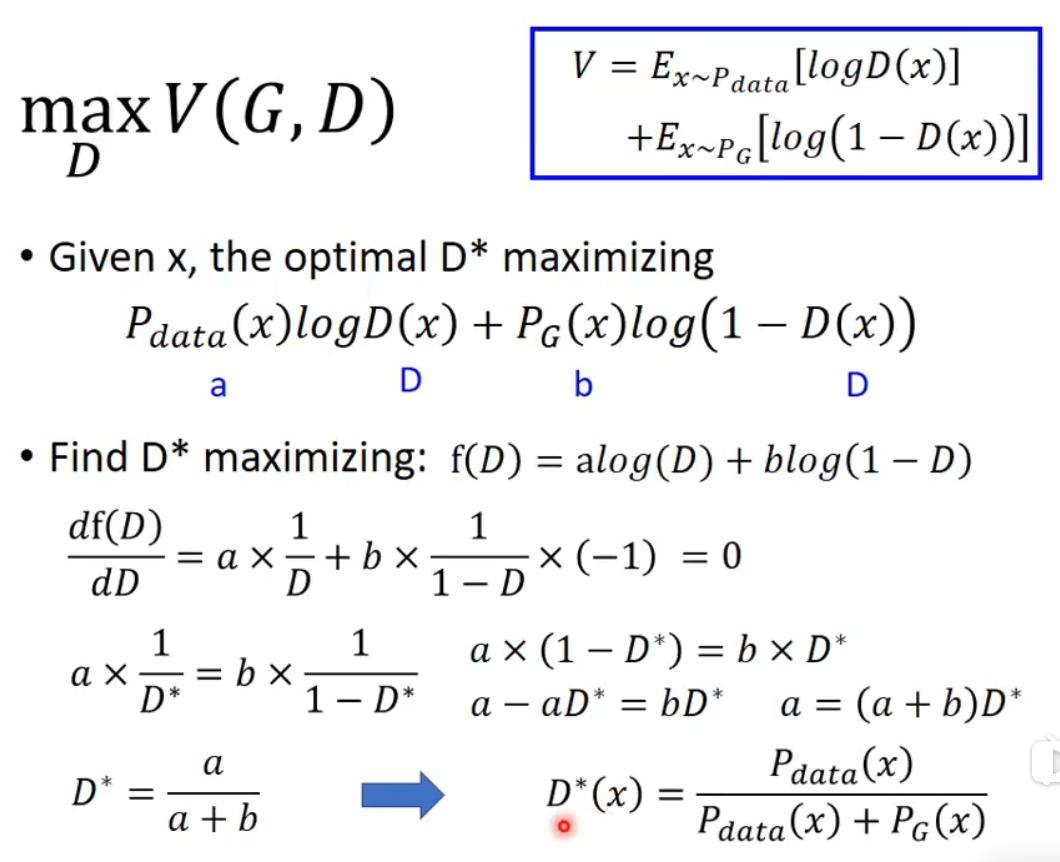
\includegraphics[scale=0.4]{screenshot006}
	\caption{}
	\label{fig:screenshot006}
	\end{figure}
	
	
	\begin{figure}[H]
	\centering
	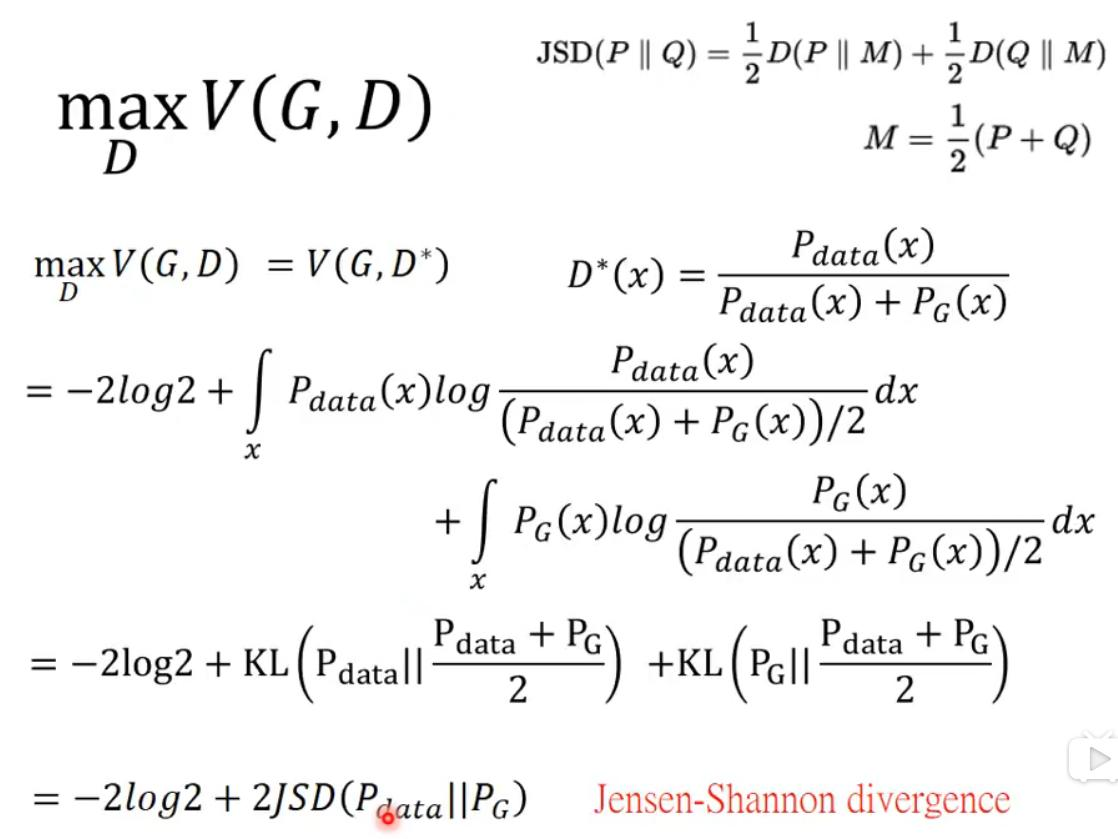
\includegraphics[scale=0.4]{screenshot007}
	\caption{}
	\label{fig:screenshot007}
	\end{figure}
	
	求解的优化问题
	\begin{figure}[H]
	\centering
	\includegraphics[scale=0.4]{screenshot008}
	\caption{}
	\label{fig:screenshot008}
	\end{figure}
	使用交替更新生成器与判别器参数的方法来求解这个minmax问题,但是无法保证收敛
	\begin{figure}[H]
	\centering
	\includegraphics[scale=0.4]{screenshot009}
	\caption{}
	\label{fig:screenshot009}
	\end{figure}
	
	在循环中,固定生成器的参数,优化判别器时,相当于在做$\max_DV(G,D)$这一步计算。
	固定判别器参数,优化生成器时,相当于在做$\min_G\max_DV(G,D)$这一步计算,但是由于这一步计算时,每次梯度下降更新后,实际上$V(G,D)$都是会变化的,所以这一步的迭代次数要较小,使得目标函数不产生较大的变化。
	\begin{figure}[H]
	\centering
	\includegraphics[scale=0.4]{screenshot010}
	\caption{}
	\label{fig:screenshot010}
	\end{figure}
	
	\begin{figure}[H]
	\centering
	\includegraphics[scale=0.4]{screenshot011}
	\caption{}
	\label{fig:screenshot011}
	\end{figure}
	
	p和q分布的差异同样可以用f-divergence来表示:
	\begin{figure}[H]
	\centering
	\includegraphics[scale=0.4]{screenshot012}
	\caption{}
	\label{fig:screenshot012}
	\end{figure}
	
	一张图片是高维空间中的一个低维流形,所以生成器的分布与真实数据分布之间的重合部分非常小,又由于在计算js散度时是通过采样估计的,重合部分就更小了。
	
	存在问题:即使图中第二个分布比第一个更好,但是js散度相等。
	\begin{figure}[H]
	\centering
	\includegraphics[scale=0.4]{screenshot013}
	\caption{}
	\label{fig:screenshot013}
	\end{figure}
	
	
	\section{tips}
	
	
	判别器当做二分类问题训练时,不能训练的太好,会造成中间部分梯度消失,所以提出LSGAN,使用线性损失函数训练判别器:
	\begin{figure}[H]
	\centering
	\includegraphics[scale=0.4]{screenshot014}
	\caption{}
	\label{fig:screenshot014}
	\end{figure}
	
	WGAN:
	\begin{figure}[H]
	\centering
	\includegraphics[scale=0.4]{screenshot016}
	\caption{}
	\label{fig:screenshot016}
	\end{figure}


	\begin{figure}[H]
	\centering
	\includegraphics[scale=0.4]{screenshot015}
	\caption{}
	\label{fig:screenshot015}
	\end{figure}

	使用推土距离能够积累优势,逐步改进,如同眼睛进化,每一次变异都是有好处的,变异才能积累。
	\begin{figure}[H]
	\centering
	\includegraphics[scale=0.4]{screenshot017}
	\caption{}
	\label{fig:screenshot017}
	\end{figure}
	
	证明过程复杂,略
	\begin{figure}[H]
	\centering
	\includegraphics[scale=0.4]{screenshot018}
	\caption{}
	\label{fig:screenshot018}
	\end{figure}
	\begin{figure}[H]
	\centering
	\includegraphics[scale=0.4]{screenshot019}
	\caption{}
	\label{fig:screenshot019}
	\end{figure}
	\begin{figure}[H]
	\centering
	\includegraphics[scale=0.4]{screenshot022}
	\caption{}
	\label{fig:screenshot022}
\end{figure}

	WGAN-GP
	\begin{figure}[H]
	\centering
	\includegraphics[scale=0.4]{screenshot020}
	\caption{}
	\label{fig:screenshot020}
	\end{figure}
	\begin{figure}[H]
	\centering
	\includegraphics[scale=0.4]{screenshot021}
	\caption{}
	\label{fig:screenshot021}
	\end{figure}
\begin{figure}[H]
\centering
\includegraphics[scale=0.4]{screenshot024}
\caption{}
\label{fig:screenshot024}
\end{figure}


\begin{figure}[H]
\centering
\includegraphics[scale=0.4]{screenshot023}
\caption{}
\label{fig:screenshot023}
\end{figure}









	
\end{document}